\documentclass[
    ngerman,
    accentcolor=3b,
    dark_mode,
    fontsize= 12pt,
    a4paper,
    aspectratio=169,
    colorback=true,
    fancy_row_colors,
    leqno,
    fleqn,
    boxarc=3pt,
    fleqn,
    % shell_escape = false, % Kompatibilität mit sharelatex
]{algoslides}

%%------------%%
%%--Packages--%%
%%------------%%

% \usepackage{audutils}
% \usepackage{fopbot}
\usepackage{booktabs}
\usepackage{fontawesome5}
% Import all Packages from Main Preamble with relative Path (buggy, list packages instead)
% \subimport*{../../}{preamble}

%%--------------------------%%
%%--Imports from Main File--%%
%%--------------------------%%

% Get Labels from Main Document using the xr-hyper Package
\externaldocument[ext:]{../main}
% Set Graphics Path, so pictures load correctly
\graphicspath{{../pictures}}

\begin{document}
    \section{Linux im Vergleich zu anderen Betriebssysteme}\label{linux-vs-other-oses}\label{Linux im Vergleich zu anderen Betriebssysteme}
    \begin{frame}
        \slidehead{}
        \begin{itemize}
            \item Open Source
            \item Privatsphäre
            \item Sicherheit
            \item Freedom of Choice
            \item Paketverwaltung
        \end{itemize}
    \end{frame}
    \subsection{Open Source}
    \begin{frame}[c]
        \slidehead{}
        \begin{columns}
            \begin{column}[c]{0.5\textwidth}
                \begin{itemize}
                    \item Der Komplette Kernel: \url{https://github.com/torvalds/linux}
                    \item Einzelne Distributionen:
                        \begin{itemize}
                            \item Arch: \url{https://github.com/archlinux}
                            \item Ubuntu: \url{https://github.com/ubuntu}
                        \end{itemize}
                    \item Lizenz: \href{https://www.gnu.org/licenses/gpl-3.0.html}{GPLv3}
                        \begin{itemize}
                            \item Alle Projekte, die den Linux-Kernel verwenden, müssen ebenfalls GPLv3 lizensiert werden.
                        \end{itemize}
                \end{itemize}
            \end{column}
            \begin{column}[c]{0.5\textwidth}
                \begin{center}
                    \fontsize{50pt}{0pt}\selectfont\faOsi{}\\[0.2cm]
                    \normalsize\textbf{Open Source}
                \end{center}
            \end{column}
        \end{columns}
    \end{frame}
    \subsection{Privatsphäre}
    \begin{frame}[c]
        \slidehead{}
        \begin{columns}
            \begin{column}[c]{0.75\textwidth}
                \centering
\includegraphics[width=0.8\textwidth]{linux_privacy.jpg}
            \end{column}
            \begin{column}[c]{0.25\textwidth}
                \begin{center}
                    \fontsize{50pt}{0pt}\selectfont\faUserSecret{}\\[0.2cm]
                    \normalsize\textbf{Privacy}
                \end{center}
            \end{column}
        \end{columns}
    \end{frame}
    \begin{frame}[c]
        \slidehead{}
        \begin{columns}
            \begin{column}[c]{0.75\textwidth}
                \begin{itemize}
                    \item Transparenz durch offenen Quellcode
                    \item Keine \enquote{Druck}, Geld mit Daten zu machen
                    \item Viele Linux-Distros legen großen Wert auf die Privatsphäre
                \end{itemize}
            \end{column}
            \begin{column}[c]{0.25\textwidth}
                \begin{center}
                    \fontsize{50pt}{0pt}\selectfont\faUserSecret{}\\[0.2cm]
                    \normalsize\textbf{Privacy}
                \end{center}
            \end{column}
        \end{columns}
    \end{frame}
    \subsection{Sicherheit}
    \begin{frame}[c]
        \slidehead{}
        \begin{columns}
            \begin{column}[c]{0.5\textwidth}
                \begin{itemize}
                    \item 97\% aller Server verwenden Linux
                    \item Wird von Großen Unternehmen mitentwickelt
                    \item Sehr fähige (Kern-) Userbase
                \end{itemize}
            \end{column}
            \begin{column}[c]{0.5\textwidth}
                \begin{center}
                    \fontsize{50pt}{0pt}\selectfont\faShield*{}\\[0.2cm]
                    \normalsize\textbf{Security}
                \end{center}
            \end{column}
        \end{columns}
    \end{frame}
    \subsection{Freedom of Choice}
    \begin{frame}[c]%
        \slidehead{}%
        \begin{columns}%
            \begin{column}[c]{0.5\textwidth}%
                \centering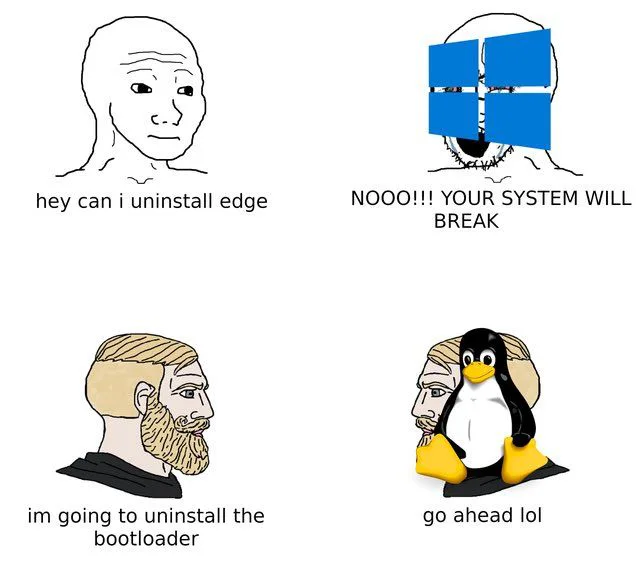
\includegraphics[height=5.5cm]{freedom_of_choice_meme.png}%
                % \centering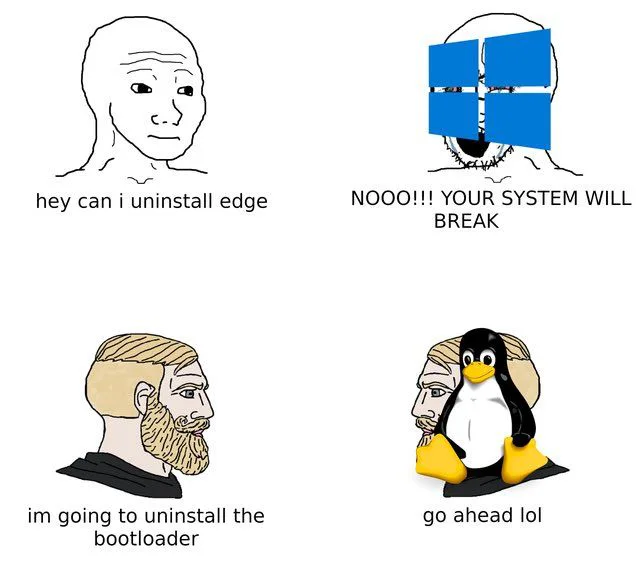
\includegraphics[width=\linewidth,height=\textheight,keepaspectratio]{freedom_of_choice_meme.png}%
            \end{column}%
            \begin{column}[c]{0.5\textwidth}
                \begin{center}
                    \fontsize{50pt}{0pt}\selectfont\faMagic{}\\[0.2cm]
                    \normalsize\textbf{Freedom of Choice}
                \end{center}
            \end{column}
        \end{columns}
    \end{frame}
\end{document}